\begin{figure}
	
	\floatbox{figure}[\FBwidth]
	{
		\caption{Months between NBER release and journal submission}\label{figure7}
	}
	{
		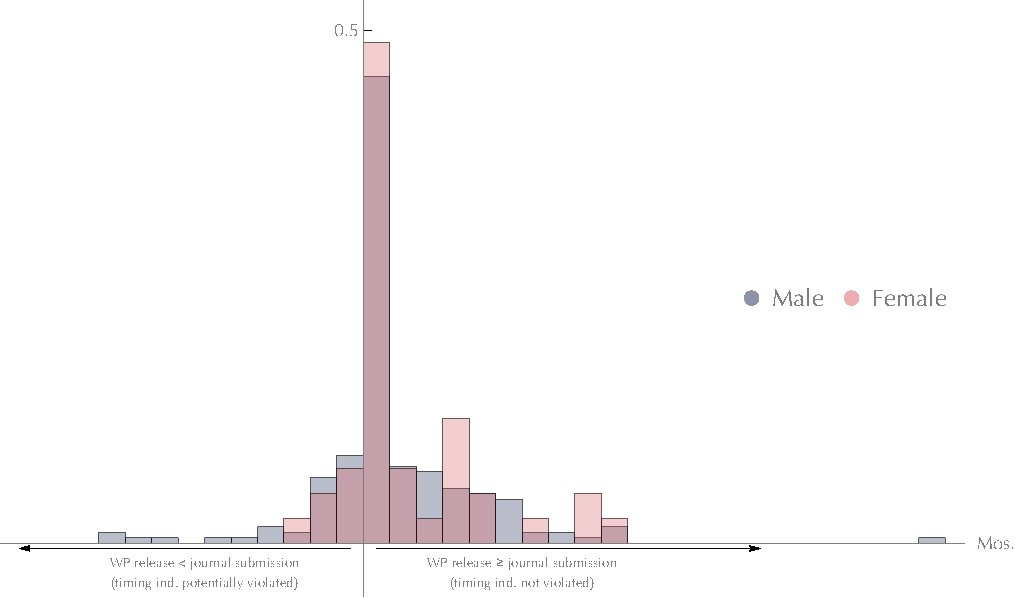
\includegraphics[width=12.3cm]{$HOME/Dropbox/Readability/draft/pdf/figure7.pdf}
		\floatfoot{\tiny \textit{Notes}. Sample 228 articles published in \textit{Econometrica}. Figure represents the distribution of the difference (in months) between a paper's release as an NBER Working Paper and submission of that same article to \textit{Econometrica} (where it is eventually published). To the right-hand side of the \(y\)-axis are articles that were released as working papers \textit{after} they they had already been submitted to \textit{Econometrica}. To the left of the \(y\)-axis are articles that were released \textit{first} as an NBER Working Paper and submitted to \textit{Econometrica} at a later date.}
	}
\end{figure}